\section{Results}\label{results}
After answering all the sub-questions, one thing is left: proving the main research question.
The main research question and its requirements were:

\textit{How to implement a transformation from typechecked Meta Casanova (MC) from the front-end, to executable code within the timeframe of the internship?}

Where the transformation must satisfy these requirements:
\begin{description}
    \item[The correctness requirement] The backend must in no case produce an incorrect program.
    \item[The .NET requirement] The executable must be able to inter-operate with .NET.
    \item[The multiplatform requirement] The generated code must run on all the platforms .NET runs on.
    \item[The performance requirement] The performance of the generated program should be better than Python.
\end{description}


\subsection{Correctness}
Unfortunately, since the front-end was incomplete, it is not possible to compile source files.
It \textit{is} however possible to write the front-end interface by hand.

\subsubsection{Data test}
The first test was developed to test the Data declarations.
It is equivalent to the following MC code.

\begin{MC}
Data int -> "::" -> List -> List
Data "nil" -> List

---------
main -> 0
\end{MC}

\subsubsection{List length test}
The list length program defined a list data structure and a program to compute its length.
This was used since it uses each basic instruction at least once, as well as matching.
It is equivalent to the following MC code:

\begin{MC}
Data int -> "::" -> List -> List
Data "nil" -> List

Func "length" -> List -> int

---------------
length nil -> 0

length xs -> res
---------------------
length x::xs -> res+1

--------------------------------
main -> length (1::2::3::4::nil)
\end{MC}

Which when executed prints \verb|4| on screen.

%This program can also be debugged with the embedded debugger.

\subsection{.NET}
The second test program was to test the .NET functionality.
It consists of a simple program that modifies XNA data structures, specifically the \verb|Vector2|.

\begin{MC}
20.0 -> x1
10.0 -> y1
Microsoft.Xna.Framework.Vector2 x1 y1 -> a
20.0 -> x2
10.0 -> y2
Microsoft.Xna.Framework.Vector2 x2 y2 -> b
Microsoft.Xna.Framework.Vector2.+ a b -> c
Microsoft.Xna.Framework.Vector2.Normalize c
y2 -> v.x 
v.x -> ret
-------------------------------------------
run -> ret
\end{MC}

Which returns \verb|20|.
This is especially interesting to debug, because we can see the values change.

\fbox{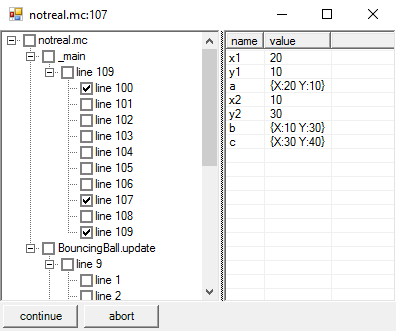
\includegraphics[width=\columnwidth-7pt]{debugger}}

\subsection{Multiplatform}
All test programs via the Microsoft .NET runtime on Windows, and on mono everywhere else.
Because no platform-specific code is used, the code runs on all platforms where mono is suported\cite{mono_platforms}.

Currently supported operating systems are:
\begin{itemize}
    \item Linux
    \item Mac OS X, iOS, tvOS, watchOS
    \item Sun Solaris
    \item BSD - OpenBSD, FreeBSD, NetBSD
    \item Microsoft Windows
    \item Nintendo Wii
    \item Sony PlayStation 3
    \item Sony PlayStation 4
\end{itemize}

\subsection{Performance}

Performance was mesured with the \textit{list length} test program.
A Python version was written to match the MC version as closely as possible:

\begin{lstlisting}[language=python]
Nil = None

def cons(x,xs):
    return (x,xs)

def length(xs):
    if xs is Nil:
        return 0
    else:
        return 1+length(xs[1])
\end{lstlisting}

Optimizations were turned off on both the C\# compiler and python, to make sure the optimizer did not take advantage of optimizations that were only applicable in this case.
This decision makes the results reflect an average program, as recursive calls are often used in MC.

The Python program counted the length of a $10^4$ element list.
To get the same precision, the MC program counted the length of a $10^6$ element list.
Both programs were executed $10^3$ times, the results below is the minimum, maximum and average time taken to count a single element.

\begin{tabular}{l|lll}
& Python & MC & Python/MC \\
\hline
min &   3442$\mu$s & 22.82$\mu$s & $151\times$ \\
max &   3627$\mu$s & 49.79$\mu$s & $72.8\times$ \\
avg &   3534$\mu$s & 36.30$\mu$s & $97.3\times$ \\
\end{tabular}

The mesurements show that MC is two orders of magnitude faster than the equivalent python code.

